\documentclass[letterpaper]{article}

%% Language and font encodings
\usepackage[english]{babel}
\usepackage[utf8x]{inputenc}
\usepackage[T1]{fontenc}

%% Sets page size and margins
\usepackage[letterpaper,top=3cm,bottom=2cm,left=2cm,right=2cm,marginparwidth=1.75cm]{geometry}

%% Useful packages
\usepackage{amsmath}
\usepackage{graphicx}
\usepackage[colorinlistoftodos]{todonotes}
\usepackage[colorlinks=true, allcolors=blue]{hyperref}
\usepackage{listings}
\usepackage{enumitem}

\usepackage[numbered,framed]{matlab-prettifier}
\let\ph\mlplaceholder % shorter macro
\lstMakeShortInline"

\lstset{
  style              = Matlab-editor,
  basicstyle         = \mlttfamily,
  escapechar         = ",
  mlshowsectionrules = true,
}

\title{EE576 HW 6}
\author{Jordan Caudill and Matt Ruffner}

\begin{document}
\maketitle

%%%%%%%%%%%%%%%%%%%%%%%%%%%%%%%%%%%%%%%%%%%%%%%%%%%%%%%%%%%%%%%%%%
%%%%%%%%%%%%%%%%%%%%%%%%%%%%%%%%%%%%%%%%%%%%%%%%%%%%%%%%%%%%%%%%%%
%%%%%%%%%%%%%%%%%%%%%%%%%%%%%%%%%%%%%%%%%%%%%%%%%%%%%%%%%%%%%%%%%%

\section{}
When the user logs in, the users DES encrypted private key is attempted to be decrypted with the supplied login password, this is then cryptographically verified against the users public key \texttt{passwd} file. A possible solution is to restrict access to \texttt{/etc/publickey} similar to \texttt{/etc/passwd}.

\section{}

The easedropper will have the following information:

\begin{enumerate}
    \item Random Challenge Number R
    \item The encrypted value of R using key J
\end{enumerate}

The question is: With this information, is it possible to guess the password using offline methods?

The answer to this question (and any encryption method) is yes because anyone could blindly guess any password with either enough patience or luck. However, the likelihood of guessing the right password is significantly lowered based on the strength of the encryption method. If the easedropper was trying to systematically figure out the password, they would need to do the following:
\begin{enumerate}
    \item Calculate the key (J) using the encrypted and unencrypted values of R.
    \item Calculate the password using the key.
\end{enumerate}

Both of these can be done given enough time, however we can look at the first step and see that if the encryption method is strong enough, it would take an unrealistic amount of time. To calculate J, you would need to take the encrypted message and figure out what was done to get J. If it was something as simple as taking $R \times J = Encryption$, then this could easily be deciphered, especially if we are given multiple data points.

Even if a person is able to calculate J, however, they would still need to figure out what its relationship is to the password. Like above, it depends on how complicated the relationship was. If it was a simple relationship, it could be guessed quite easily, especially if we can see multiple examples. However, if the relationship is not so straightforward, we would be forced to guess and this greatly lowers the probability of successfully getting the password.

\newpage
\section{}

\begin{enumerate}[label=\alph*.]
    \item We can calculate the number of false alarms by looking at the total number of transactions (100,000,000) and multiplying it by the rate at which a false alarm will occur. We can interpret a false alarm as being a time in which a real transaction triggered an alarm when it shouldn't have (0.001) as well as a time when a false transaction didn't trigger an alarm (0.09). The equation is a follows: 
    \begin{align}
    alarms_f &= transactions \times (rate_p + rate_n)\\
        &= 100,000,000 \times (0.001 + 0.09) \\
        &= 9,100,000
    \end{align}
    9,100,000 false alarms will occur.
    
    \item To calculate the number of true alarms, we need to take the number of hacking attemps (1000) and multiply it by the number of true alarms, which we can calculate by taking the number of false alarms and subtracting it from 1 (1-0.09). We get the following:
    \begin{align}
    alarms_t &= attempts \times (1 - rate_n)\\
        &= 100,000,000 \times (1 - 0.09) \\
        &= 910
    \end{align}
    910 true alarms will occur.
    
    \item To calculate the number of hacking attempts will go unnoticed, we can take the total number of hacking attempts (1000) and subtract the number of true alarms (910). We get the following:
    \begin{align}
    undetected &= attempts - detected\\
        &= 1,000 - 910 \\
        &= 90
    \end{align}
    90 attacks will go unnoticed
\end{enumerate}



\section{}
The file with permissions \texttt{644} is world readable, so if the filename and absolute path are known, it can be accessed even though the directory is listed with permissions \texttt{730} and is not accessbible by users outside the owner's group.



\section{}

\begin{itemize}
    \item \textbf{No access for group and other}: An advantage of this scheme is it is very secure and files are only accessible by the creator. A disadvantage is sharing files with others is difficult and would require modification of each file after creation. A scenario where this would be preferable is for private user file such as private keys for SSH authentication.
    
    
    \item \textbf{Read/execute access for group and none for other}: This is the most common scheme and is advantageous because it is common for users to be in groups where some files are shared. This may not be desirable in the case where there is a malicious user in or has added themselves to the creating user's group. This is appropriate for medium-sensitivity documents such as per-user web pages.
    
    \item \textbf{Read/execute access for group and other}: This is the least secure file creation mode and makes sharing files between others but also imposes no restrictions on which users outside the creator's group may access and or execute it. This can be useful for system wide informational file such as non-system-critical logs and temp files which are accessible by anyone.
\end{itemize}

\newpage
\section{DeterLab}
\begin{figure}[h!]
    \centering
    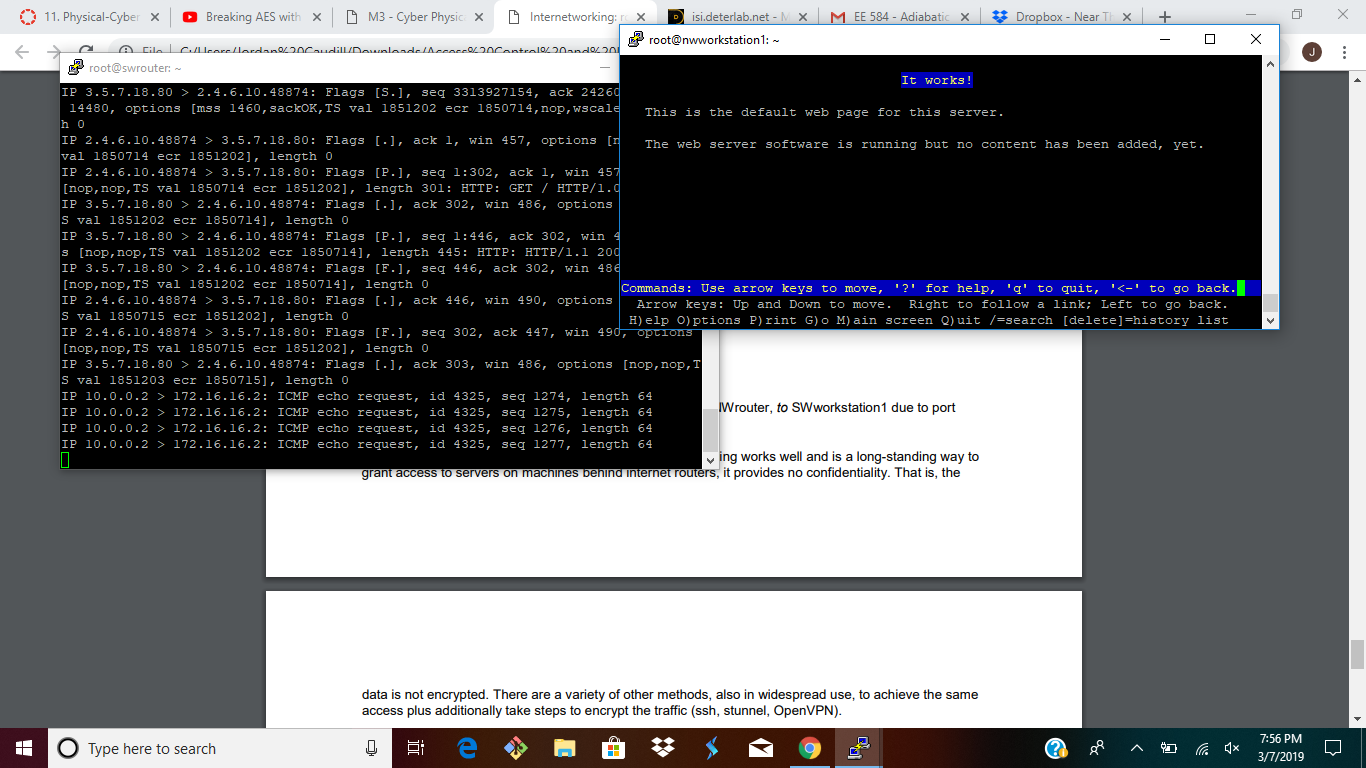
\includegraphics[width=\textwidth]{576HW6.png}
    \caption{screenshot}
    \label{fig:my_label}
\end{figure}




\end{document}